%!TEX TS-program = xelatex
%!TEX encoding = UTF-8 Unicode
%!TeX spellcheck = it_IT
%!TEX root = ../tesi.tex

\chapter{Applicativi}\label{chap:applicativi}
\section{Network Simulator 3}\label{sec:ns-3}
Network Simulator 3 (ns-3)~\cite{ns3Website} è un simulatore a eventi discreti utilizzato principalmente in ambito accademico e di ricerca,
scritto in \Cpp{} e Python; è un software libero distribuito sotto licenza GNU GPLv2.
Creato nel 2006 da un gruppo coordinato da Tom Henderson, George Riley, Sally Floyd e Sumit Roy con lo scopo
di ovviare ad alcune grosse limitazioni della precedente versione (ns-2), come ad esempio la necessità di utilizzare
un linguaggio di \textit{scripting} dedicato per modellare le simulazioni o una maggiore scalabilità~\cite{Henderson:2006:NPG:1190455.1190468}.
Attualmente è l'unica versione della serie a essere sviluppata.
È d'obbligo menzionare che, sebbene tutte le versione siano state scritte in \Cpp, ns-3 non è retrocompatibile i precedenti.
%
% \begin{figure}[htbp]
% 	\centering
% 		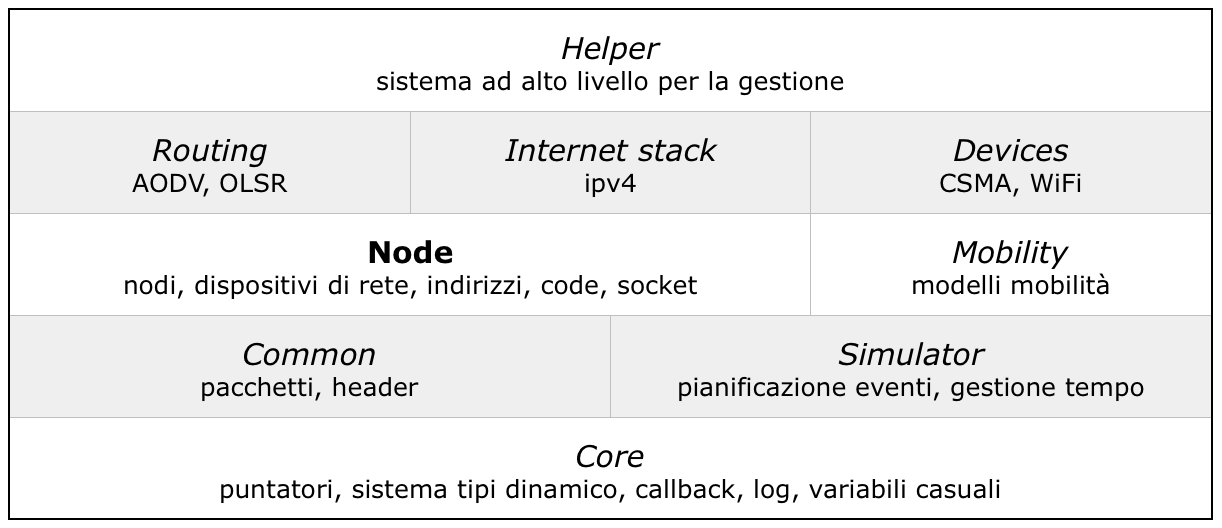
\includegraphics[width=.8\textwidth]{struttura-ns3.png}
% \caption{Panoramica della struttura interna di ns-3.\label{fig:struttura-ns3}}
% \end{figure}
%
\paragraph{Elementi chiave}
In ns-3, il dispositivo di elaborazione di base (unità elementare) è chiamato \textit{nodo}
e fornisce i metodi per gestire i dispositivi nelle simulazioni;
Può essere paragonato a un computer a cui è possibile aggiungere funzionalità come applicazioni,
stack protocollari e schede periferiche.
Sui nodi sono eseguite delle attività per raggiungere uno scopo, le \textit{applicazioni};
Per esempio, le applicazioni \textsf{UdpEchoClientApplication} e \textsf{UdpEchoServerApplication} compongono
un'aplicazione client/server per gestire e scambiare pacchetti nella rete.
Le comunicazioni fra i nodi avvengono tramite degli speciali \textit{canali};
questi possono essere definiti dallo sviluppatore e permettono di modellare concetti semplici come un collegamento su cavo
fino a quelli più complessi come uno \textit{switch Ethernet}.
Su un nodo è possibile installare uno o più \textit{dispositivi di rete} che permettono la comunicazione con altri nodi attraverso i canali.
Un nodo può essere connesso a più canali attraverso diversi dispositivi di rete.
La simulazione di una grande rete obbliga lo sviluppatore a creare migliaia di nodi, dispositivi di rete e canali.
Per facilitare questo tipo di operazioni molto comuni sono state inserite nel simulatore degli agenti, chiamati \textit{Helper}.
%
\paragraph{Struttura di una simulazione}
Per creare una semplice simulazione è necessario:
\begin{itemize}
	\item impostare gli argomenti che saranno letti da riga di comando;
	\item impostare il valore degli attributi delle classi;
	\item creare i nodi;
	\item configurare il livello fisico e MAC;
	\item impostare il livello di rete, il protocollo di routing e gli indirizzi;
	\item configurare e installare le applicazioni;
	\item impostare la poszione iniziale dei nodi e l'eventuale mobilità;
	\item pianificare eventuali eventi definiti dall'utente;
	\item avviare la simulazione.
\end{itemize}
%
\section{\SUMO}\label{sec:sumo}
\SUMO~\cite{SUMO2012} è un simulatore per traffico veicolare su larga scala; è \textit{open source}, scritto in \Cpp
e distribuito sotto licenza Eclipse Public V2.
Al suo interno si trovano diversi applicativi utili, dall'importazione di dati reali alla creazione di percorsi
per pedoni, diverse tipologie di veicoli, eccetera.
Proprio queste \textit{utility} sono state utilizzate per l'elaborazione delle informazioni sugli edifici (fornite poi
al modello \textit{Obstacle Shadowing}) e il posizionamento dei veicoli.
%
% \subsection{Realizzazione degli scenari}
Per creare uno scenario derivato da un ambiente reale, come quelli che saranno utilizzati nelle simulazioni,
e poterlo utilizzare in ns-3, sono necessarie alcune elaborazioni intermedie.

Il primo passo consiste nell'utilizzare la piattaforma gratuita OpenStreetMap (OSM)~\cite{osmWebsite} per
ottenere le informazioni sul mondo reale (Figura~\ref{fig:esempio-file-osm}) e da queste estrarre i dati sugli ostacoli.
Il file ottenuto viene convertito dall'\textit{utiliy} di SUMO Polyconvert che si occupa di tradure alcune informazioni
sugli ostacoli, come per esempio convertire la posizione da coordinate geografiche a cartesiane;
il file risultante conterrà i poligoni che saranno letti dal modulo \textit{Obstacle Shadowing}) (Figura~\ref{fig:esempio-file-poly}).
Il secondo passo è la generazione delle posizioni dei veicoli.
A questo scopo è stato creato uno \textit{script} apposito che, sfruttando le librerie per Python messe a disposizione
nel pacchetto di SUMO, partendo da un punto e percorrendo le strade ammissibili posiziona i veicoli a una certa distanza.
L'articolo originale~\cite{Carpenter:2015:OMI:2756509.2756512} utilizzava una funzione già presente in SUMO
per il posizionamento casuale che però, non permettendo di specificare una distanza fra i veicoli, non andava bene per gli scenari desiderati in questo lavoro.
%
Il file ottenuto dal processo viene convertito in un formato per ns-2 tramite lo \textit{script} traceExporter (sempre compreso nell pacchetto SUMO)
e questo sarà poi eseguito dal modulo di ns-3 \textsf{Ns2MobilityHelper} in modo da posizionare i nodi durante la simulazione.
Il processo completo è riassunto nella Figura~\ref{fig:generazione-file-sumo}.

Il pacchetto SUMO include anche un'interfaccia grafica per visualizzare le simuazion (Figura~\ref{fig:esempio-file-poly}).
% TODO: provare a stampare per vedere come si vedono le immagini !
%
\begin{figure}[htbp]
	\centering
		\fbox{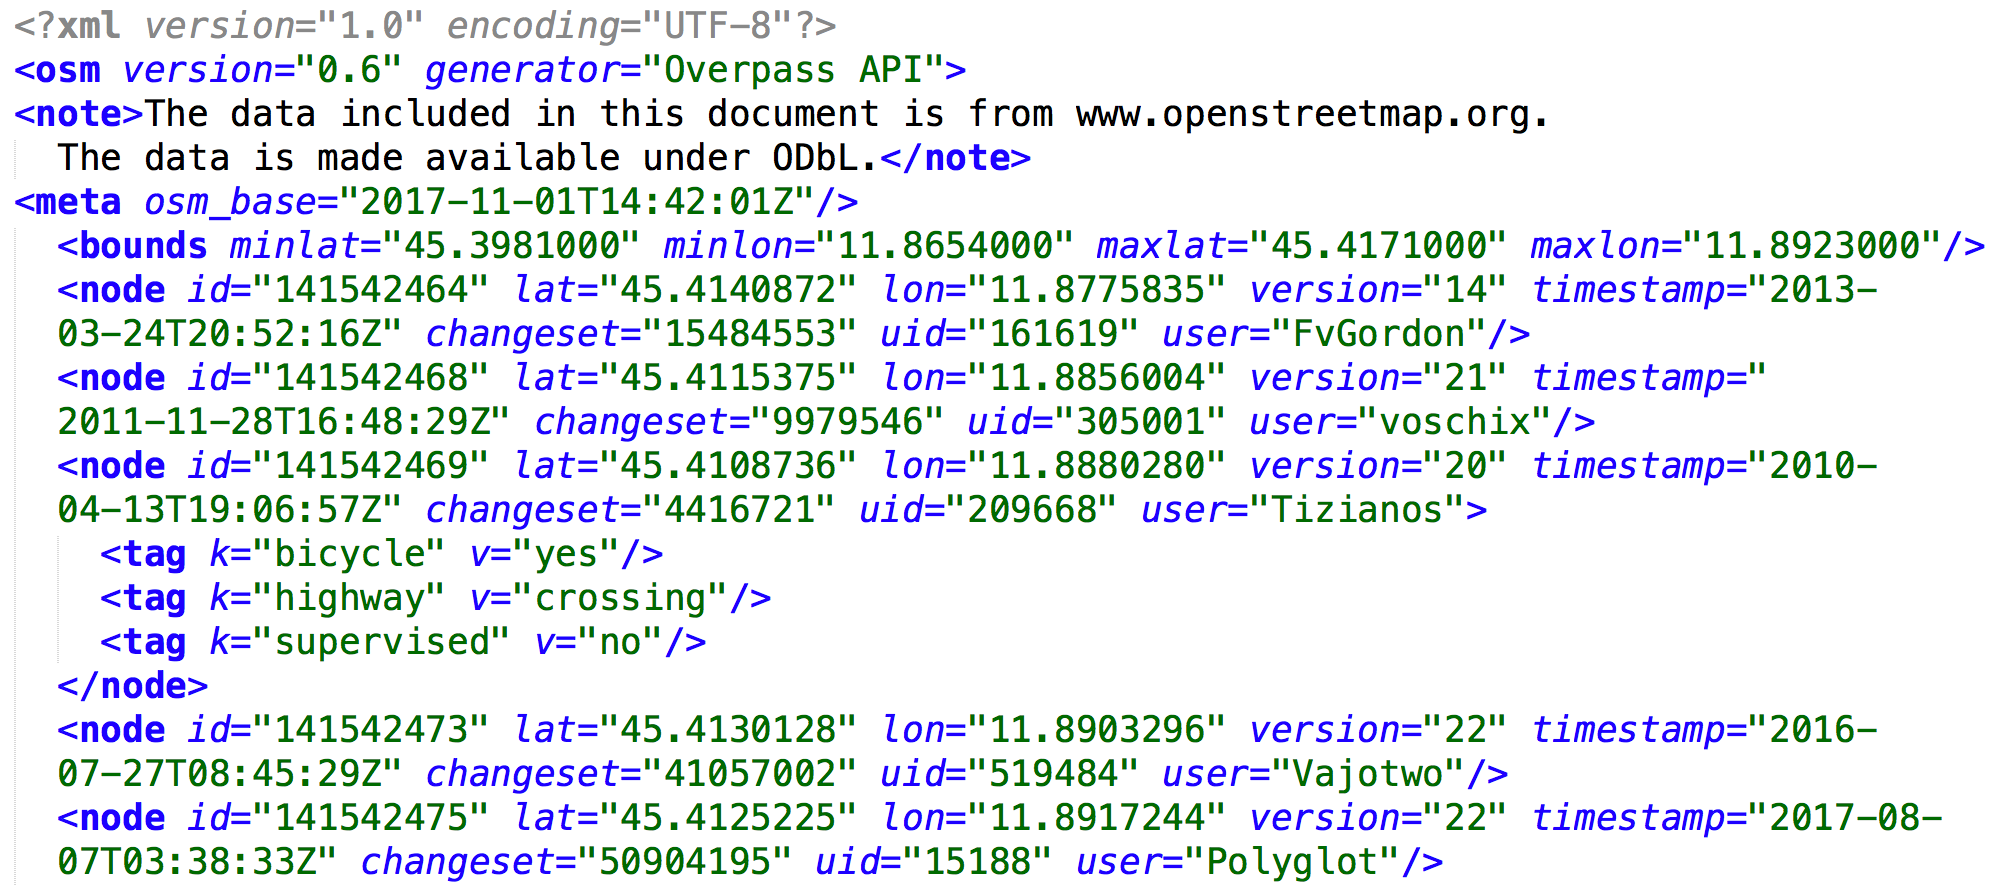
\includegraphics[width=\textwidth]{file-osm-dettaglio.png}}
\caption{Un estratto del file dati sugli edifici dopo la conversione con Polyconvert.\label{fig:esempio-file-osm}}
\end{figure}
%
%
\begin{figure}[htbp]
	\centering
		\fbox{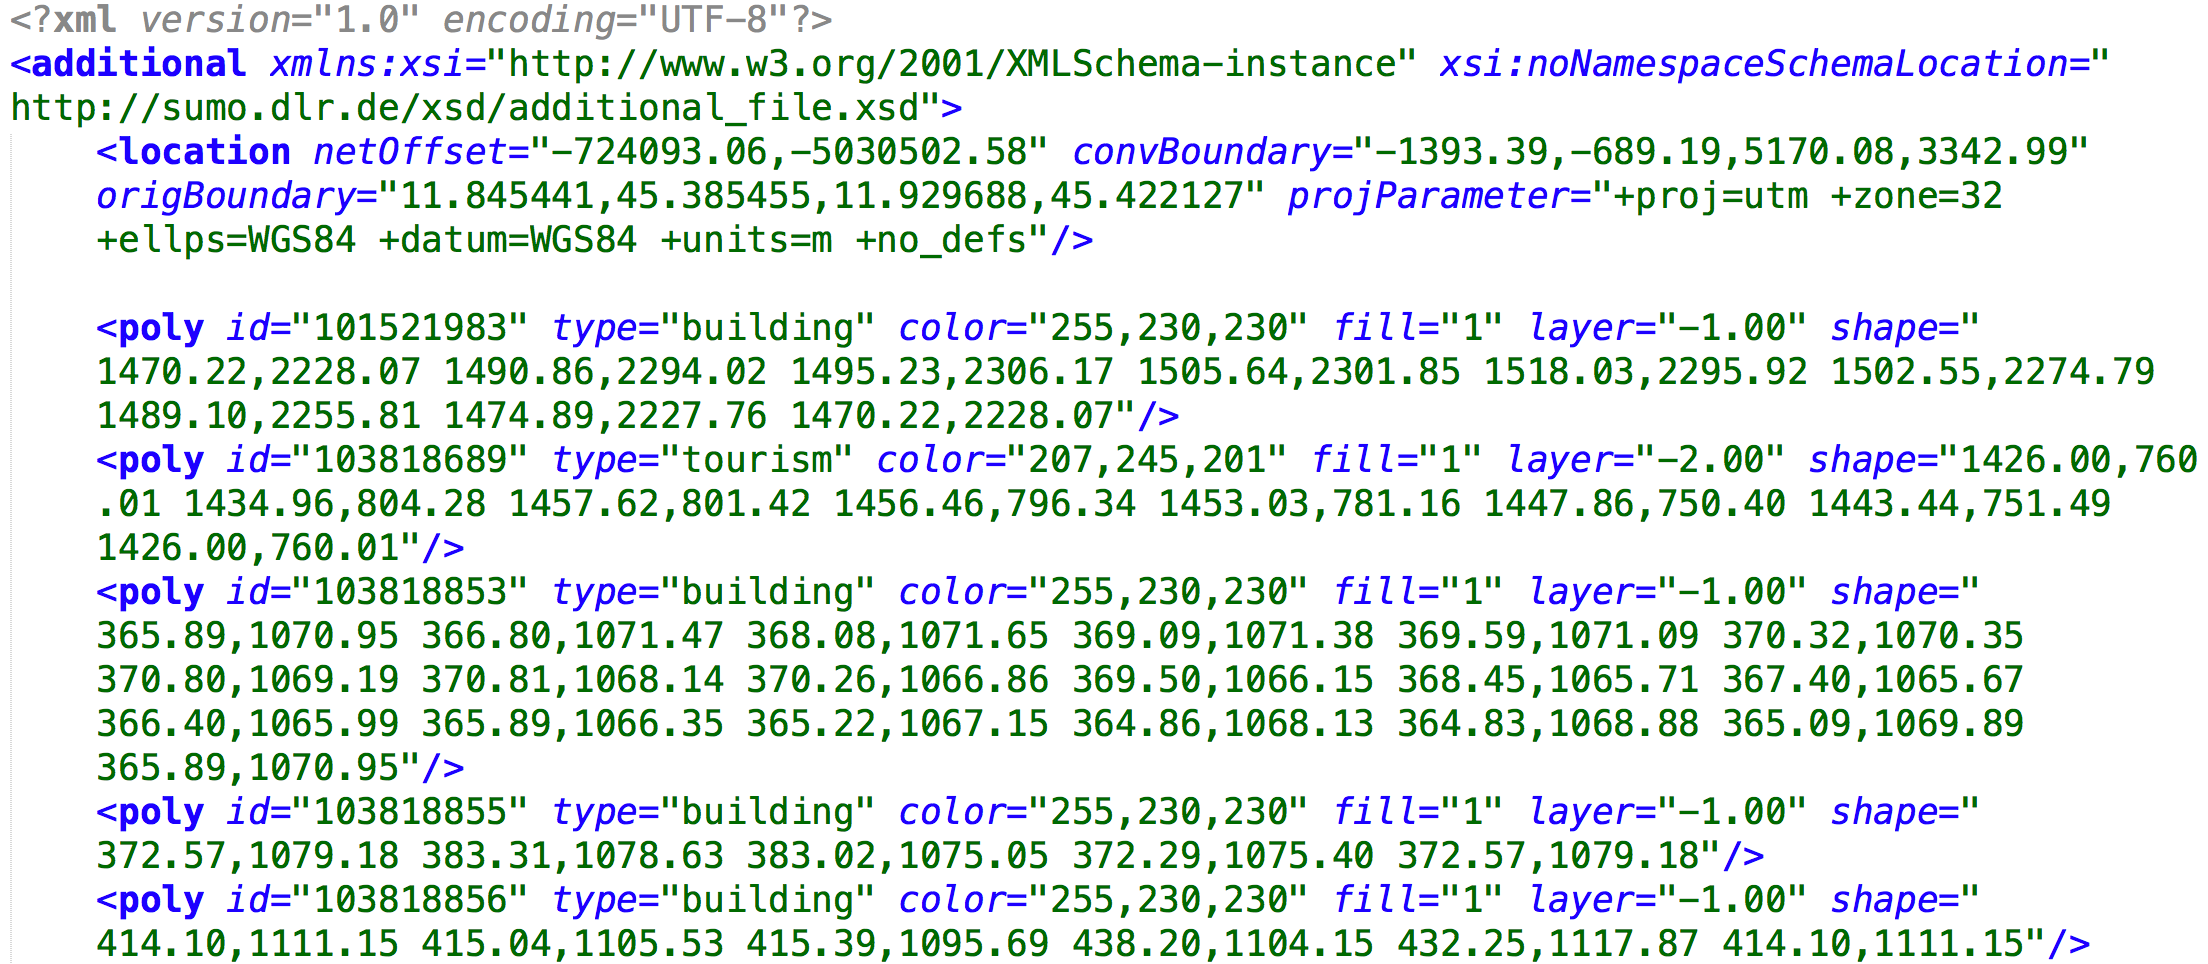
\includegraphics[width=\textwidth]{file-poly-dettaglio.png}}
\caption{Un estratto del file dati sugli edifici dopo la conversione con Polyconvert.\label{fig:esempio-file-poly}}
\end{figure}
%
\begin{figure}[htbp]
	\centering
		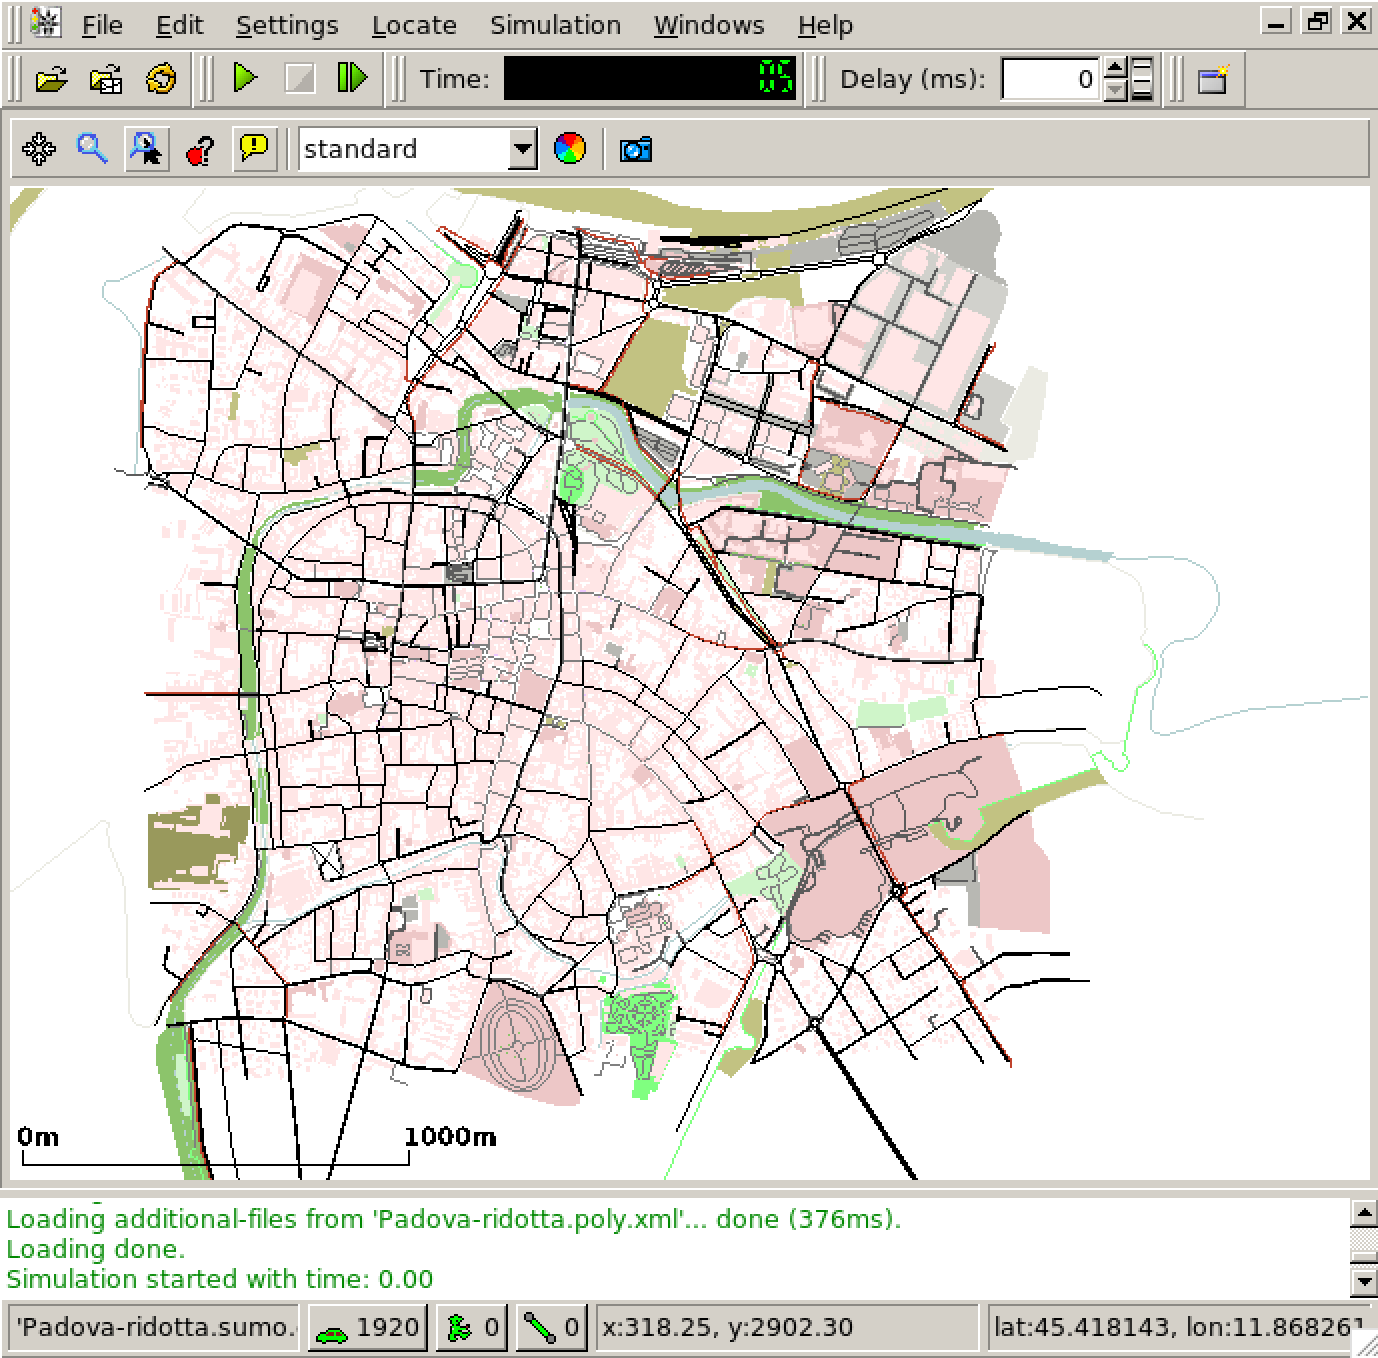
\includegraphics[width=.49\textwidth]{sumo-gui-pd-estesa.png}
		\hfill
		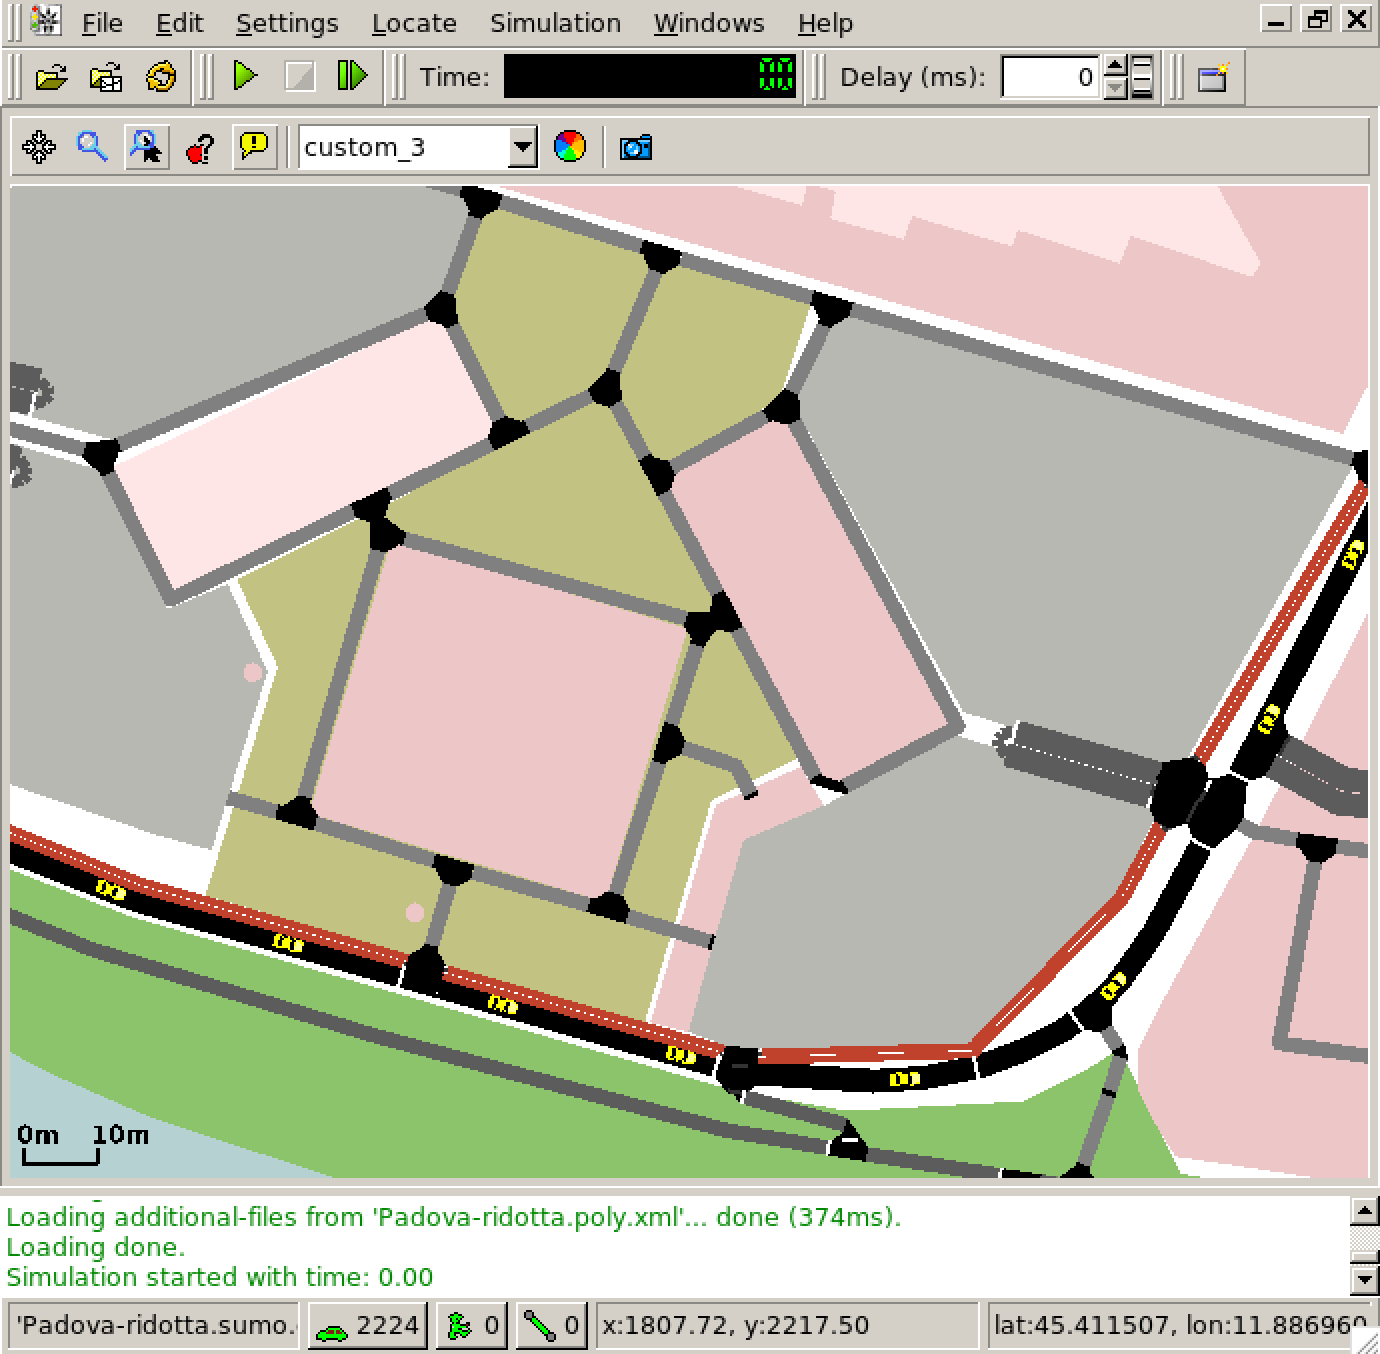
\includegraphics[width=.49\textwidth]{sumo-gui-pd-dettaglio.png}
\caption{Scenario urbano raffigurante il centro di Padova (IT) simulato con SUMO; a destra un dettaglio con i veicoli presenti.\label{fig:sumo-gui}}
\end{figure}
%
% Generazione figura con: https://www.easel.ly/create?id=https://s3.amazonaws.com/easel.ly/all_easels/3240510/1510073603&key=pri
\begin{figure}[htbp]
	\centering
	{
		\setlength{\fboxsep}{0pt}	% override default setting
		\fbox{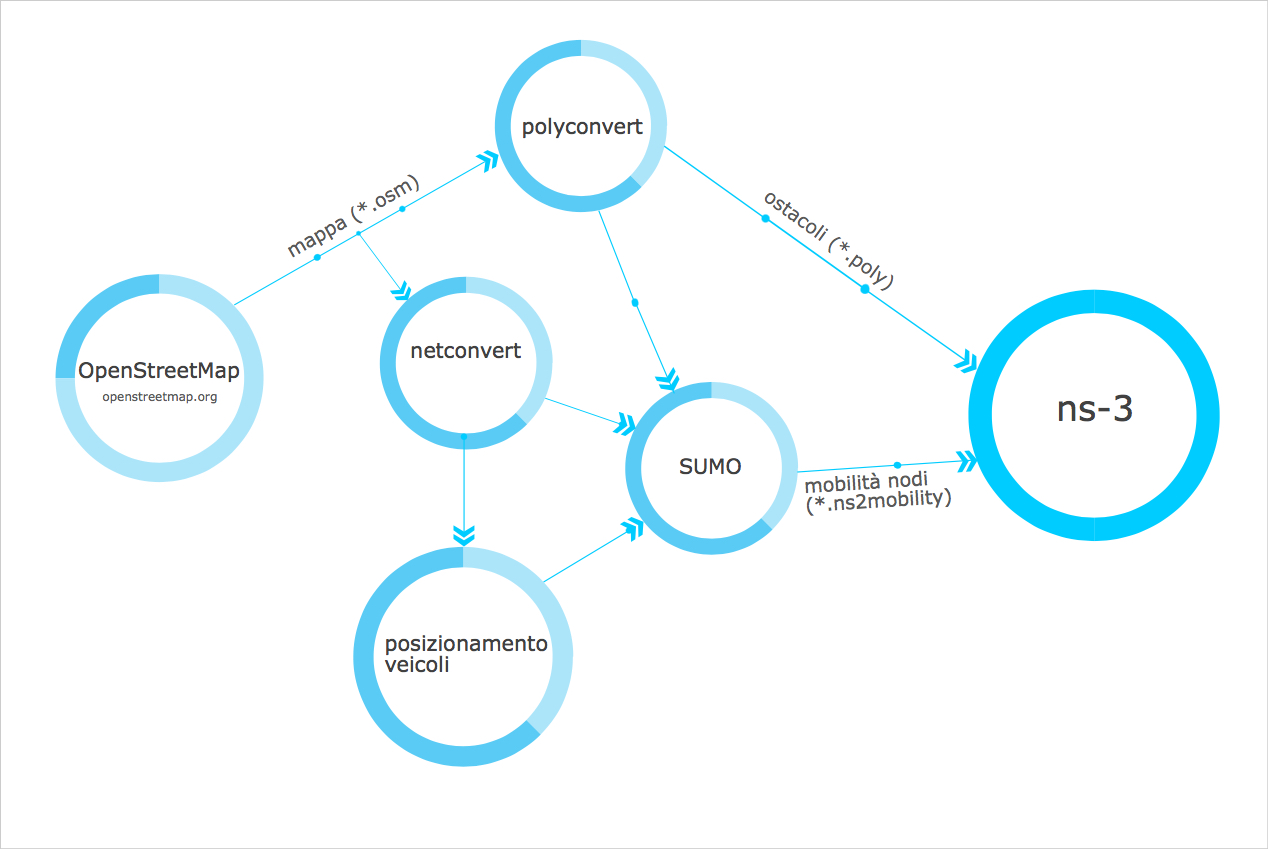
\includegraphics[width=.9\textwidth]{generazione-file-sumo.jpg}}
	}
\caption{Procedimento per estrarre le informazioni da OSM e generare i file per la simulazione con ns-3.\label{fig:generazione-file-sumo}}
\end{figure}
